\subsection{Amplificador de potencia}

En primer lugar identificamos la etapa del amplificador de potencias en el diagrama del amplificador multietapas, la cual es la que contiene a los transistores $Q4$, $Q5$ y $Q6$. Dicha etapa se muestra en la figura \ref{fig:met-etapa-amplificador-de-potencia}.

\begin{figure}[ht]
    \centering
    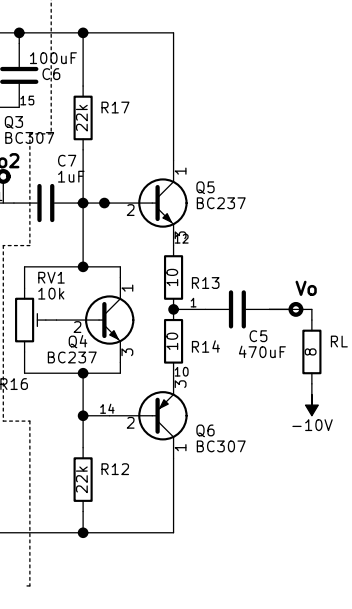
\includegraphics[width=0.23\textwidth]{src/images/metodología/etapa-de-potencia.png}
    \caption{Etapa del amplificador de potencia}
    \label{fig:met-etapa-amplificador-de-potencia}
\end{figure}

Ahora procedemos a calcular los puntos estáticos de operación, para ello tomamos los capacitores como circuitos abiertos, ya que estamos trabajando en DC y empezamos a calcular las corrientes en el transistor $Q4$.

Asumiremos que las corrientes de base $I_{bQ5}$ e $I_{bQ6}$ son muy pequeñas en comparación con la corriente $I_{R17}$ por tanto la tomaremos como despreciables.

Ahora aplicando LCK en el multiplicador de voltaje ($Q_4$):
\begin{equation}
I_{RV1} + I_{cQ4} = I_{R17}    
\end{equation}

Si ahora asumimos $I_bQ4$ despreciable:

\begin{equation}
    I_{RV1} = \frac{V_{BEQ4}}{XR_{V1}}
\end{equation}

Aplicando LVK tenemos:

\begin{equation}
    V_{CEQ4} = I_{RV1} * R_v1
\end{equation}

Usando (2) y (3):

$$ V_{CEQ4} = \frac{V_{BEQ4}}{X*R_{V1}} * R_{V!}$$

\begin{equation}
    V_{CEQ4} = \frac{V_{BEQ4}}{X}
\end{equation}

Debido a que el amplificador es de clase AB el voltaje $V_{CEQ4}$ tiene que ser dos veces el voltaje base emisor $V_{be}$ para los transistores $Q5$ y $Q6$ estén lo más cerca posible de la zona activa y se pueda reducir el efecto crossover de la salida.

Aplicando LVK entre las dos referencias tenemos:

$$10V - R_{17}*I_{17} - 2V_{beQ4} - R_{12}*I_{17} + 10V = 0$$

despejando $I_{17}$:

\begin{equation}
    I_{17} = \frac{20 - 2V_{beQ4}}{R_{17} + R_{12}}
\end{equation}

Usando (1), (2) y (5) tenemos:

\begin{equation}
    I_{cQ4} = \frac{20 - 2V_{beQ4}}{R_{17} + R_{12}} - \frac{2V_{beQ4}}{R_{V1}}
    \label{eq:icQ4}
\end{equation}

Usando la ecuacion (\ref{eq:icQ4}) y los datos:

$V_{beQ4} = 0.62 V$ 

$R_{17} = R_{12} = 22k\Omega$ :

$R_{V1} = 10k\Omega$ 

$$    I_{cQ4} = \frac{20 - 2 * 0.62 V}{22k\Omega + 22k\Omega} - \frac{2 * 0.62 V}{10 k\Omega} $$

$$ I_{cQ4} = 302.36 \mu A$$

Tomando $hfe_{Q4} = 230$

\begin{equation}
    I_{bQ4} = I_{cQ4} / hfe
\end{equation}

$$ I_{bQ4} = 1.31 \mu A$$

$$ V_{ceQ4} = 2 * 0.62 V = 1.24 V$$

Ahora, volviendo a despreciar las corriente de base y aplicando LVK en la malla con los transistores

$$V_{ceQ4} - V_{beQ5} - I_{eQ5}* (R_{13} + R_{14}) - V_{beQ6} = 0$$

despejando $I_{eQ5}$

\begin{equation}
    I_{eQ5} =\frac{ V_{ceQ4} - V_{beQ5} - V_{beQ6} }{R_{13} + R_{14}}
\end{equation}

Tomando $V_{beQ5} = V_{beQ4} = 0.62 V$ y $V_{beQ6} = 0.55 V$, entonces: 

$$I_{eQ5} = \frac{ 1.24 V - 0.62 V - 0.55 V }{10 \Omega + 10 \Omega }$$

$$ I_{eQ5} = I_{eQ6} \approx I_{cQ5} \approx I_{cQ6} = 350\mu A$$

Basado en las I de emisor ahora calulamos las corrientes de base, asumiendo que $hfe_{Q5} = 230 $ y $hfe_{Q6} = 150$

$$I_{bQ5} = I_{cQ5} / hfe = 350\mu A / 230 = 1.52 \mu A $$

$$I_{bQ6} = I_{cQ6} / hfe = 350\mu A / 150 = 2.33 \mu A $$

Se asume que $V_{ceQ5} = V_{ceQ6} $, por tanto:

$$ 10 - 2 V_{ceQ5} - (R_{14} + R_{13}) * I_{eQ5} + 10 = 0$$

despejando $V_{ceQ5}$ tenemos:

\begin{equation}
    V_{ceQ5} = V_{ceQ6} = \frac{ 20 - (R_{14} + R_{13}) * I_{eQ5} }{2}
\end{equation}

por tanto 

$$ V_{ceQ5} = V_{ceQ6} = \frac{ 20 V - (10 + 10) \Omega * 350\mu A }{2} = 9.99 V$$

El resumén de los puntos estáticos de operación del amplificador de potencia se muestran en la tabla \ref{tab:amplificador-de-potencia-puntos-estaticos}.

\begin{table}[ht]
    \centering
    \begin{tabular}{|c|c|c|}
        \hline
        Transistor & \textbf{$I_c$} & \textbf{$V_{ce}$} \\
        \hline
        $Q4$ & $302.36 \mu A$ & $1.24 V$ \\
        $Q5$ & $350\mu A$ & $9.99 V$ \\
        $Q6$ & $350\mu A$ & $9.99 V$ \\
        \hline
    \end{tabular}
    \caption{Puntos estáticos de operación del amplificador de potencia}
    \label{tab:amplificador-de-potencia-puntos-estaticos}
\end{table}

A continuación, en la figura \ref{fig:met-puntos-estaticos-amplificador-de-potencia} se muestran los puntos estáticos de operación del amplificador de potencia.

\begin{figure}[ht]
    \centering
    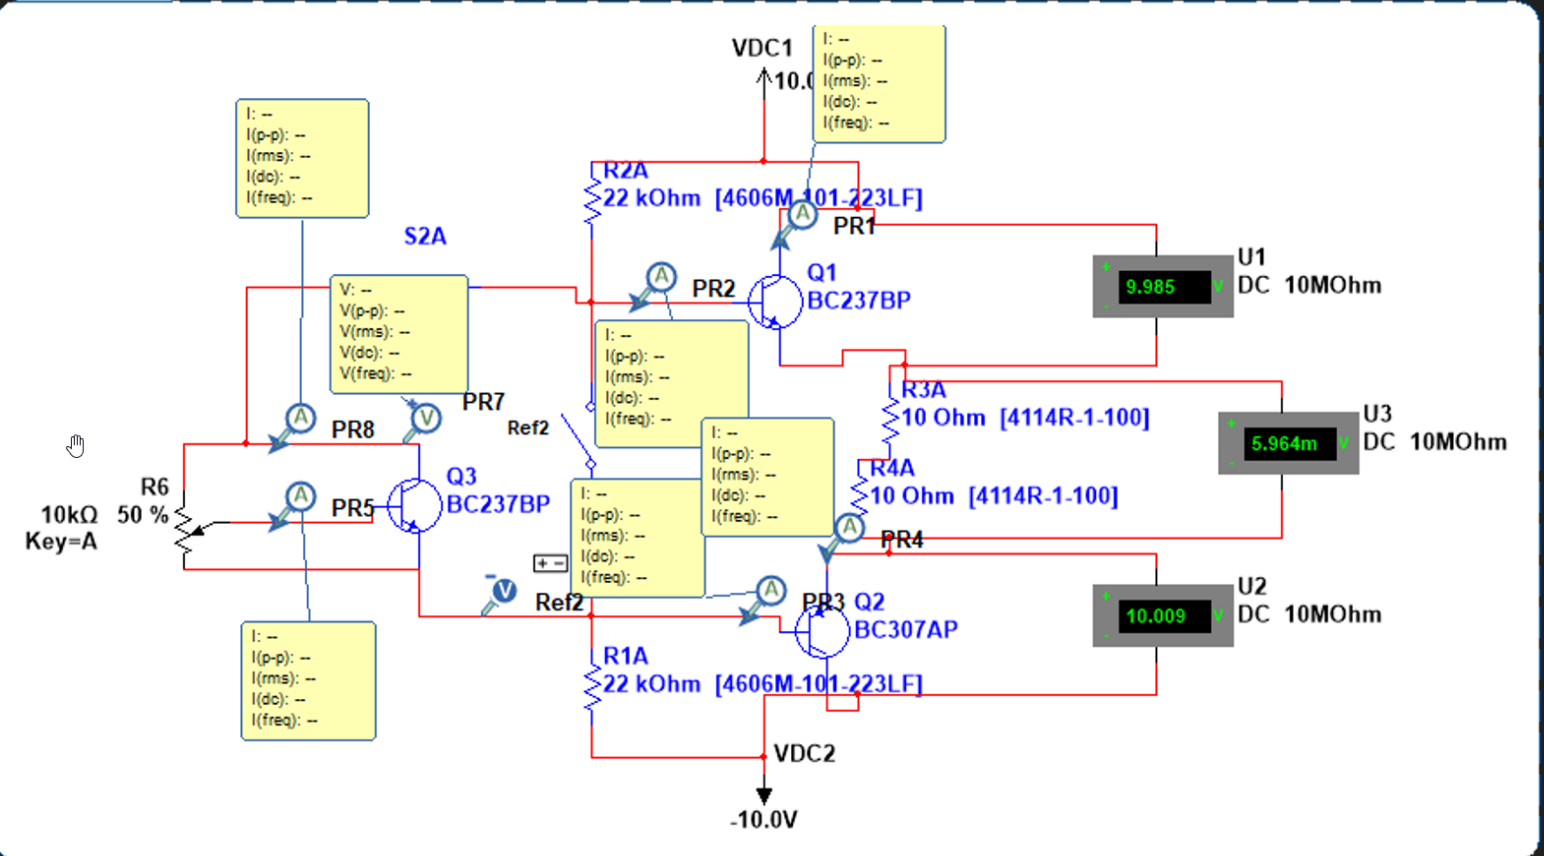
\includegraphics[width=0.9\textwidth]{src/images/metodología/simulacion-etapa-potencia-puntos-estaticos.png}
    \caption{Puntos estáticos de operación del amplificador de potencia}
    \label{fig:met-puntos-estaticos-amplificador-de-potencia}
\end{figure}

Ahora, para la parte dinámica, calculamos los parámetros del transistor utilizando $V_t = 26 mV$ y $V_A = 100 V$

$$gm = \frac{I_c}{V_t} = \frac{0,35 mA}{26 mV}$$

$$gm = 13.46 mS$$

$$R_\pi = \frac{\beta}{gm} = \frac{230}{13.46\times 10^{-3}}$$

$$ R_\pi = 17.07k \Omega$$

$$ R_o = \frac{V_A}{I_c} = \frac{100 V}{0,35 mA} = 285,71 k\Omega$$

Obtenidos los parámetros dinámicos podemos calcular la ganancia del amplificador hacinedo un análisis de las corrientes de entrada y salida del circuito, obteniendo la expresión:

 $$ A = \frac{(1 + gmr_{\pi5})(r_{13} + r_l)r_L}{[r_{\pi 5} + (1 + gmr\pi5)(r_{13} + r_L)](r_{13} + r_L)}$$

 $$A = 0.96 $$

 Ahora, para calcular la impedancia de entrada:

 $$ Z_i = r_{17} \parallel r{12} \parallel [r_{\pi5} + (1 + gmr_{\pi 5})(r_{13} + r_l)] $$
 
 $$ Z_i = 10.77K\Omega $$

 Mientras que la impedancia de salida viene dada por la expresión:

$$ Z_o = r_{13} + \frac{r_{\pi5} + r_{17}/2}{1 + gmr_{\pi5}} $$

 $$ Z_o = 132 \Omega$$

 El modelo dinámico del amplificador de potencia se muestra en la tabla \ref{tab:met-amp-potencia-modelo-dinamico}.

\begin{table}[ht]
    \centering
    \begin{tabular}{|c|c|}
        \hline
        parámetro & valor  \\
        \hline
        $Z_i$ & $10.77k\Omega$ \\
        \hline
        $Z_o$ & $132\Omega$ \\
        \hline
        $A$ & $0.96$ \\
        \hline
    \end{tabular}
    \caption{Modelo dinámico del amplificador de potencia}
    \label{tab:met-amp-potencia-modelo-dinamico}
\end{table}

en la figura \ref{fig:sim-amp-potencia-ganancia} se muestra la ganancia del amplificador de potencia. Se puede observar que el voltaje de entrada y de salida se superponen, ya que la ganancia es aproximadamente 1.

\begin{figure}[ht]
    \centering
    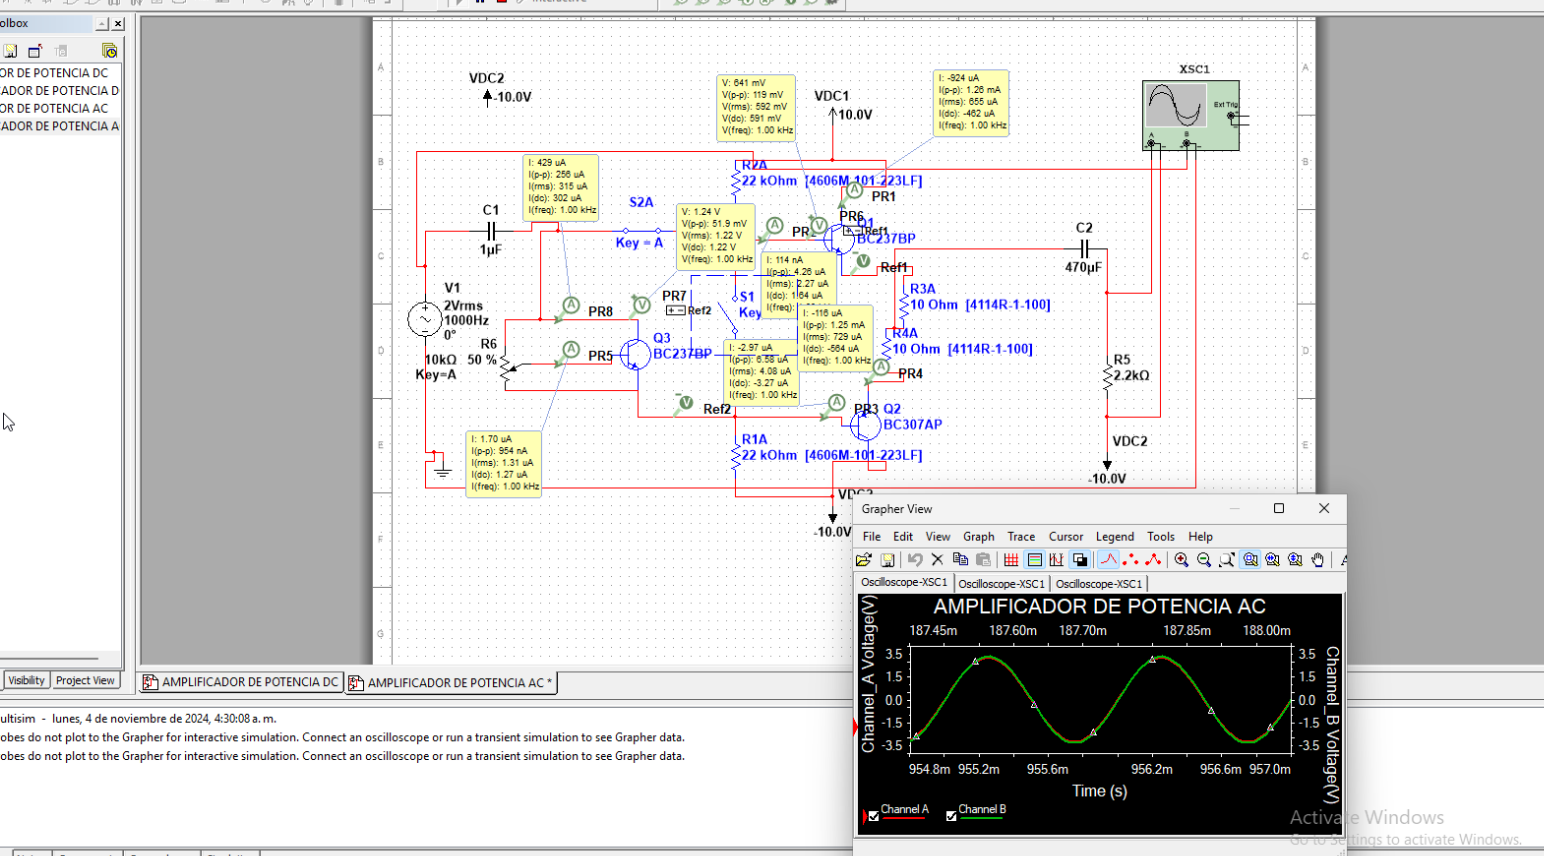
\includegraphics[width=0.9\textwidth]{src/images/p1/p1-sim-ganancia.png}
    \caption{Ganancia del amplificador de potencia}
    \label{fig:sim-amp-potencia-ganancia}
\end{figure}

En la figura \ref{fig:sim-amp-potencia-efecto-crossover} se muestra el efecto crossover del amplificador de potencia. 

\begin{figure}[ht]
    \centering
    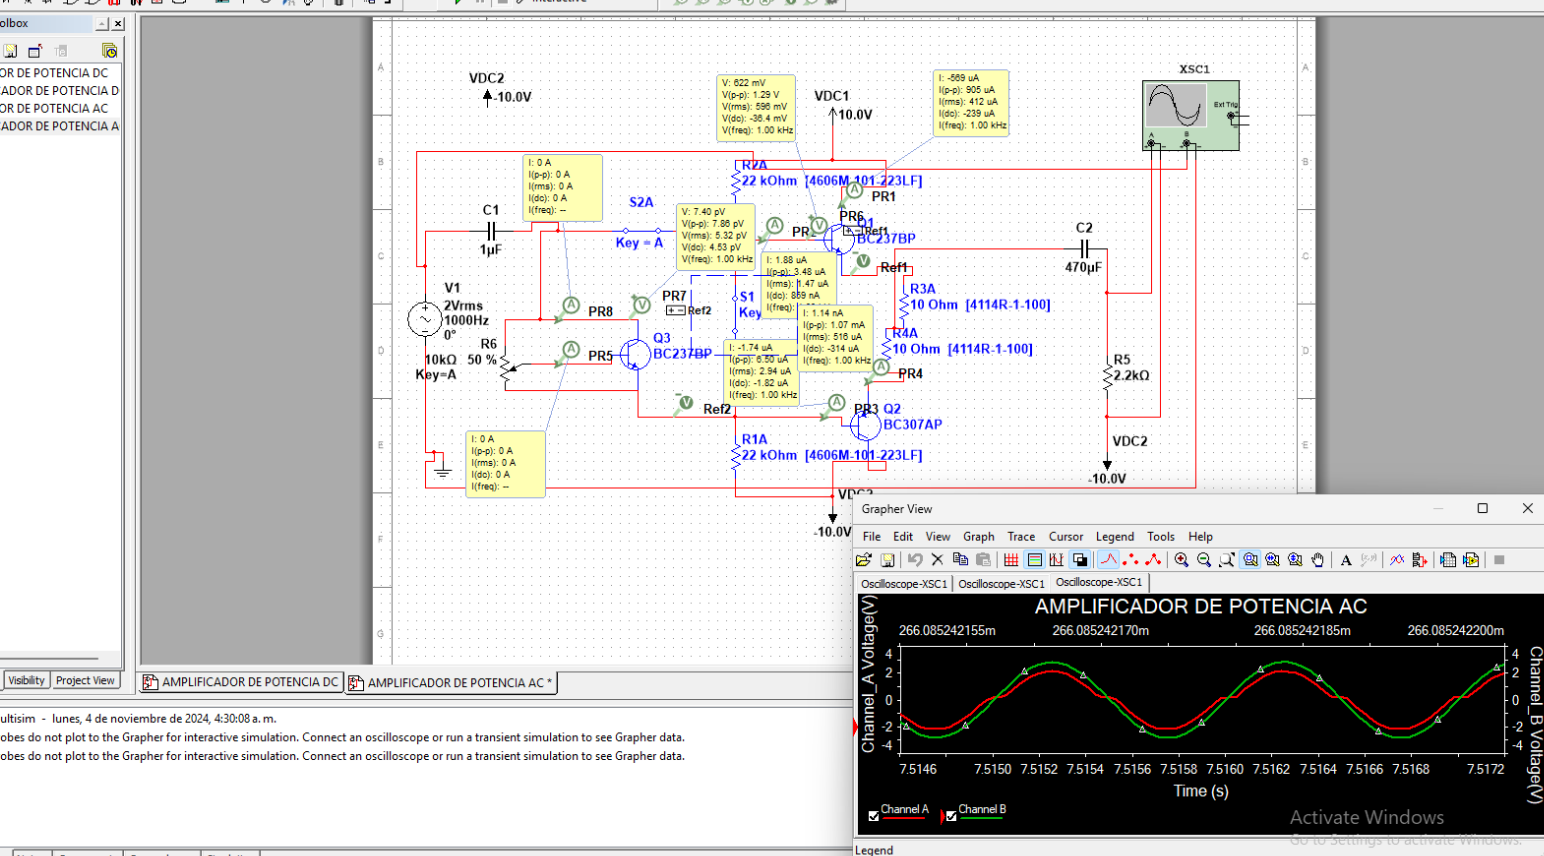
\includegraphics[width=0.9\textwidth]{src/images/p1/p1-sim-efecto-crossover.png}
    \caption{Efecto crossover del amplificador de potencia}
    \label{fig:sim-amp-potencia-efecto-crossover}
\end{figure}